% !TEX program = xelatex
\documentclass[tikz, crop, border = {2pt 2pt 2pt 2pt}]{standalone}

\usepackage{concmath-otf}
\usetikzlibrary{calc, angles, quotes, patterns}
\usetikzlibrary{decorations.pathreplacing, decorations.pathmorphing, calligraphy}

\usepackage{xcolor}
\definecolor{c1}{HTML}{7B1D6E}
\definecolor{c2}{HTML}{DB3977}
\definecolor{c3}{HTML}{F0736D}
\definecolor{c4}{HTML}{FEB14C}
\definecolor{c5}{HTML}{7AB561}
\definecolor{c6}{HTML}{46AD9F}
\definecolor{c7}{HTML}{04708A}
\definecolor{c8}{HTML}{0D4A70}

\begin{document}
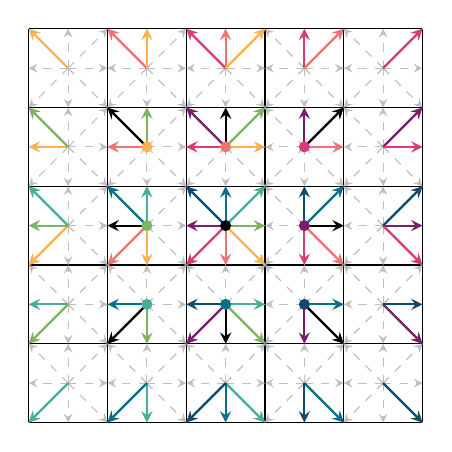
\begin{tikzpicture}
	\draw (0, 0) grid (5, 5);

	\foreach \i in {0.5, 1.5, 2.5, 3.5, 4.5} {
			\foreach \j in {0.5, 1.5, 2.5, 3.5, 4.5} {
					\coordinate (x) at (\i, \j);
					\draw[thin, dashed, lightgray, -stealth] (x)-- ++ (1/2, 0);
					\draw[thin, dashed, lightgray, -stealth] (x)-- ++ (0, 1/2);
					\draw[thin, dashed, lightgray, -stealth] (x)-- ++ (-1/2, 0);
					\draw[thin, dashed, lightgray, -stealth] (x)-- ++ (0, -1/2);
					\draw[thin, dashed, lightgray, -stealth] (x)-- ++ (1/2, 1/2);
					\draw[thin, dashed, lightgray, -stealth] (x)-- ++ (-1/2, 1/2);
					\draw[thin, dashed, lightgray, -stealth] (x)-- ++ (-1/2, -1/2);
					\draw[thin, dashed, lightgray, -stealth] (x)-- ++ (1/2, -1/2);
				}
		}

	\def\cs{2pt}
	\coordinate (x) at (2.5, 2.5);
	\draw[thick, -stealth] ($(x) + (1, 0)$) -- ++ (1/2, 0);
	\draw[thick, -stealth] ($(x) + (0, 1)$) -- ++ (0, 1/2);
	\draw[thick, -stealth] ($(x) + (-1, 0)$) -- ++ (-1/2, 0);
	\draw[thick, -stealth] ($(x) + (0, -1)$) -- ++ (0, -1/2);
	\draw[thick, -stealth] ($(x) + (1, 1)$) -- ++ (1/2, 1/2);
	\draw[thick, -stealth] ($(x) + (-1, 1)$) -- ++ (-1/2, 1/2);
	\draw[thick, -stealth] ($(x) + (-1, -1)$) -- ++ (-1/2, -1/2);
	\draw[thick, -stealth] ($(x) + (1, -1)$) -- ++ (1/2, -1/2);

	\coordinate (x) at (3.5, 2.5);
	\draw[c1, thick, -stealth] ($(x) + (1, 0)$) -- ++ (1/2, 0);
	\draw[c1, thick, -stealth] ($(x) + (0, 1)$) -- ++ (0, 1/2);
	\draw[c1, thick, -stealth] ($(x) + (-1, 0)$) -- ++ (-1/2, 0);
	\draw[c1, thick, -stealth] ($(x) + (0, -1)$) -- ++ (0, -1/2);
	\draw[c1, thick, -stealth] ($(x) + (1, 1)$) -- ++ (1/2, 1/2);
	\draw[c1, thick, -stealth] ($(x) + (-1, 1)$) -- ++ (-1/2, 1/2);
	\draw[c1, thick, -stealth] ($(x) + (-1, -1)$) -- ++ (-1/2, -1/2);
	\draw[c1, thick, -stealth] ($(x) + (1, -1)$) -- ++ (1/2, -1/2);

	\coordinate (x) at (3.5, 3.5);
	\draw[c2, thick, -stealth] ($(x) + (1, 0)$) -- ++ (1/2, 0);
	\draw[c2, thick, -stealth] ($(x) + (0, 1)$) -- ++ (0, 1/2);
	\draw[c2, thick, -stealth] ($(x) + (-1, 0)$) -- ++ (-1/2, 0);
	\draw[c2, thick, -stealth] ($(x) + (0, -1)$) -- ++ (0, -1/2);
	\draw[c2, thick, -stealth] ($(x) + (1, 1)$) -- ++ (1/2, 1/2);
	\draw[c2, thick, -stealth] ($(x) + (-1, 1)$) -- ++ (-1/2, 1/2);
	\draw[c2, thick, -stealth] ($(x) + (-1, -1)$) -- ++ (-1/2, -1/2);
	\draw[c2, thick, -stealth] ($(x) + (1, -1)$) -- ++ (1/2, -1/2);

	\coordinate (x) at (2.5, 3.5);
	\draw[c3, thick, -stealth] ($(x) + (1, 0)$) -- ++ (1/2, 0);
	\draw[c3, thick, -stealth] ($(x) + (0, 1)$) -- ++ (0, 1/2);
	\draw[c3, thick, -stealth] ($(x) + (-1, 0)$) -- ++ (-1/2, 0);
	\draw[c3, thick, -stealth] ($(x) + (0, -1)$) -- ++ (0, -1/2);
	\draw[c3, thick, -stealth] ($(x) + (1, 1)$) -- ++ (1/2, 1/2);
	\draw[c3, thick, -stealth] ($(x) + (-1, 1)$) -- ++ (-1/2, 1/2);
	\draw[c3, thick, -stealth] ($(x) + (-1, -1)$) -- ++ (-1/2, -1/2);
	\draw[c3, thick, -stealth] ($(x) + (1, -1)$) -- ++ (1/2, -1/2);

	\coordinate (x) at (1.5, 3.5);
	\draw[c4, thick, -stealth] ($(x) + (1, 0)$) -- ++ (1/2, 0);
	\draw[c4, thick, -stealth] ($(x) + (0, 1)$) -- ++ (0, 1/2);
	\draw[c4, thick, -stealth] ($(x) + (-1, 0)$) -- ++ (-1/2, 0);
	\draw[c4, thick, -stealth] ($(x) + (0, -1)$) -- ++ (0, -1/2);
	\draw[c4, thick, -stealth] ($(x) + (1, 1)$) -- ++ (1/2, 1/2);
	\draw[c4, thick, -stealth] ($(x) + (-1, 1)$) -- ++ (-1/2, 1/2);
	\draw[c4, thick, -stealth] ($(x) + (-1, -1)$) -- ++ (-1/2, -1/2);
	\draw[c4, thick, -stealth] ($(x) + (1, -1)$) -- ++ (1/2, -1/2);

	\coordinate (x) at (1.5, 2.5);
	\draw[c5, thick, -stealth] ($(x) + (1, 0)$) -- ++ (1/2, 0);
	\draw[c5, thick, -stealth] ($(x) + (0, 1)$) -- ++ (0, 1/2);
	\draw[c5, thick, -stealth] ($(x) + (-1, 0)$) -- ++ (-1/2, 0);
	\draw[c5, thick, -stealth] ($(x) + (0, -1)$) -- ++ (0, -1/2);
	\draw[c5, thick, -stealth] ($(x) + (1, 1)$) -- ++ (1/2, 1/2);
	\draw[c5, thick, -stealth] ($(x) + (-1, 1)$) -- ++ (-1/2, 1/2);
	\draw[c5, thick, -stealth] ($(x) + (-1, -1)$) -- ++ (-1/2, -1/2);
	\draw[c5, thick, -stealth] ($(x) + (1, -1)$) -- ++ (1/2, -1/2);

	\coordinate (x) at (1.5, 1.5);
	\draw[c6, thick, -stealth] ($(x) + (1, 0)$) -- ++ (1/2, 0);
	\draw[c6, thick, -stealth] ($(x) + (0, 1)$) -- ++ (0, 1/2);
	\draw[c6, thick, -stealth] ($(x) + (-1, 0)$) -- ++ (-1/2, 0);
	\draw[c6, thick, -stealth] ($(x) + (0, -1)$) -- ++ (0, -1/2);
	\draw[c6, thick, -stealth] ($(x) + (1, 1)$) -- ++ (1/2, 1/2);
	\draw[c6, thick, -stealth] ($(x) + (-1, 1)$) -- ++ (-1/2, 1/2);
	\draw[c6, thick, -stealth] ($(x) + (-1, -1)$) -- ++ (-1/2, -1/2);
	\draw[c6, thick, -stealth] ($(x) + (1, -1)$) -- ++ (1/2, -1/2);

	\coordinate (x) at (2.5, 1.5);
	\draw[c7, thick, -stealth] ($(x) + (1, 0)$) -- ++ (1/2, 0);
	\draw[c7, thick, -stealth] ($(x) + (0, 1)$) -- ++ (0, 1/2);
	\draw[c7, thick, -stealth] ($(x) + (-1, 0)$) -- ++ (-1/2, 0);
	\draw[c7, thick, -stealth] ($(x) + (0, -1)$) -- ++ (0, -1/2);
	\draw[c7, thick, -stealth] ($(x) + (1, 1)$) -- ++ (1/2, 1/2);
	\draw[c7, thick, -stealth] ($(x) + (-1, 1)$) -- ++ (-1/2, 1/2);
	\draw[c7, thick, -stealth] ($(x) + (-1, -1)$) -- ++ (-1/2, -1/2);
	\draw[c7, thick, -stealth] ($(x) + (1, -1)$) -- ++ (1/2, -1/2);

	\coordinate (x) at (3.5, 1.5);
	\draw[c8, thick, -stealth] ($(x) + (1, 0)$) -- ++ (1/2, 0);
	\draw[c8, thick, -stealth] ($(x) + (0, 1)$) -- ++ (0, 1/2);
	\draw[c8, thick, -stealth] ($(x) + (-1, 0)$) -- ++ (-1/2, 0);
	\draw[c8, thick, -stealth] ($(x) + (0, -1)$) -- ++ (0, -1/2);
	\draw[c8, thick, -stealth] ($(x) + (1, 1)$) -- ++ (1/2, 1/2);
	\draw[c8, thick, -stealth] ($(x) + (-1, 1)$) -- ++ (-1/2, 1/2);
	\draw[c8, thick, -stealth] ($(x) + (-1, -1)$) -- ++ (-1/2, -1/2);
	\draw[c8, thick, -stealth] ($(x) + (1, -1)$) -- ++ (1/2, -1/2);

	\fill[black] (2.5, 2.5) circle (\cs);
	\fill[c1] (3.5, 2.5) circle (\cs);
	\fill[c2] (3.5, 3.5) circle (\cs);
	\fill[c3] (2.5, 3.5) circle (\cs);
	\fill[c4] (1.5, 3.5) circle (\cs);
	\fill[c5] (1.5, 2.5) circle (\cs);
	\fill[c6] (1.5, 1.5) circle (\cs);
	\fill[c7] (2.5, 1.5) circle (\cs);
	\fill[c8] (3.5, 1.5) circle (\cs);
\end{tikzpicture}
\end{document}
